% CDFG of predict() — Data Glove Review 2, Figure 2 (v3: named operations, no IDs)
% Compile: pdflatex cdfg.tex && pdftoppm -png -r 300 cdfg.pdf cdfg
\documentclass[border=8pt]{standalone}
\usepackage{tikz}
\usetikzlibrary{shapes.geometric,arrows.meta,positioning,fit,backgrounds,calc}

\definecolor{opfill}{HTML}{E8F0FE}
\definecolor{decfill}{HTML}{FDE8E8}
\definecolor{bb}{HTML}{F7F7F2}
\definecolor{edge}{HTML}{333333}

\begin{document}
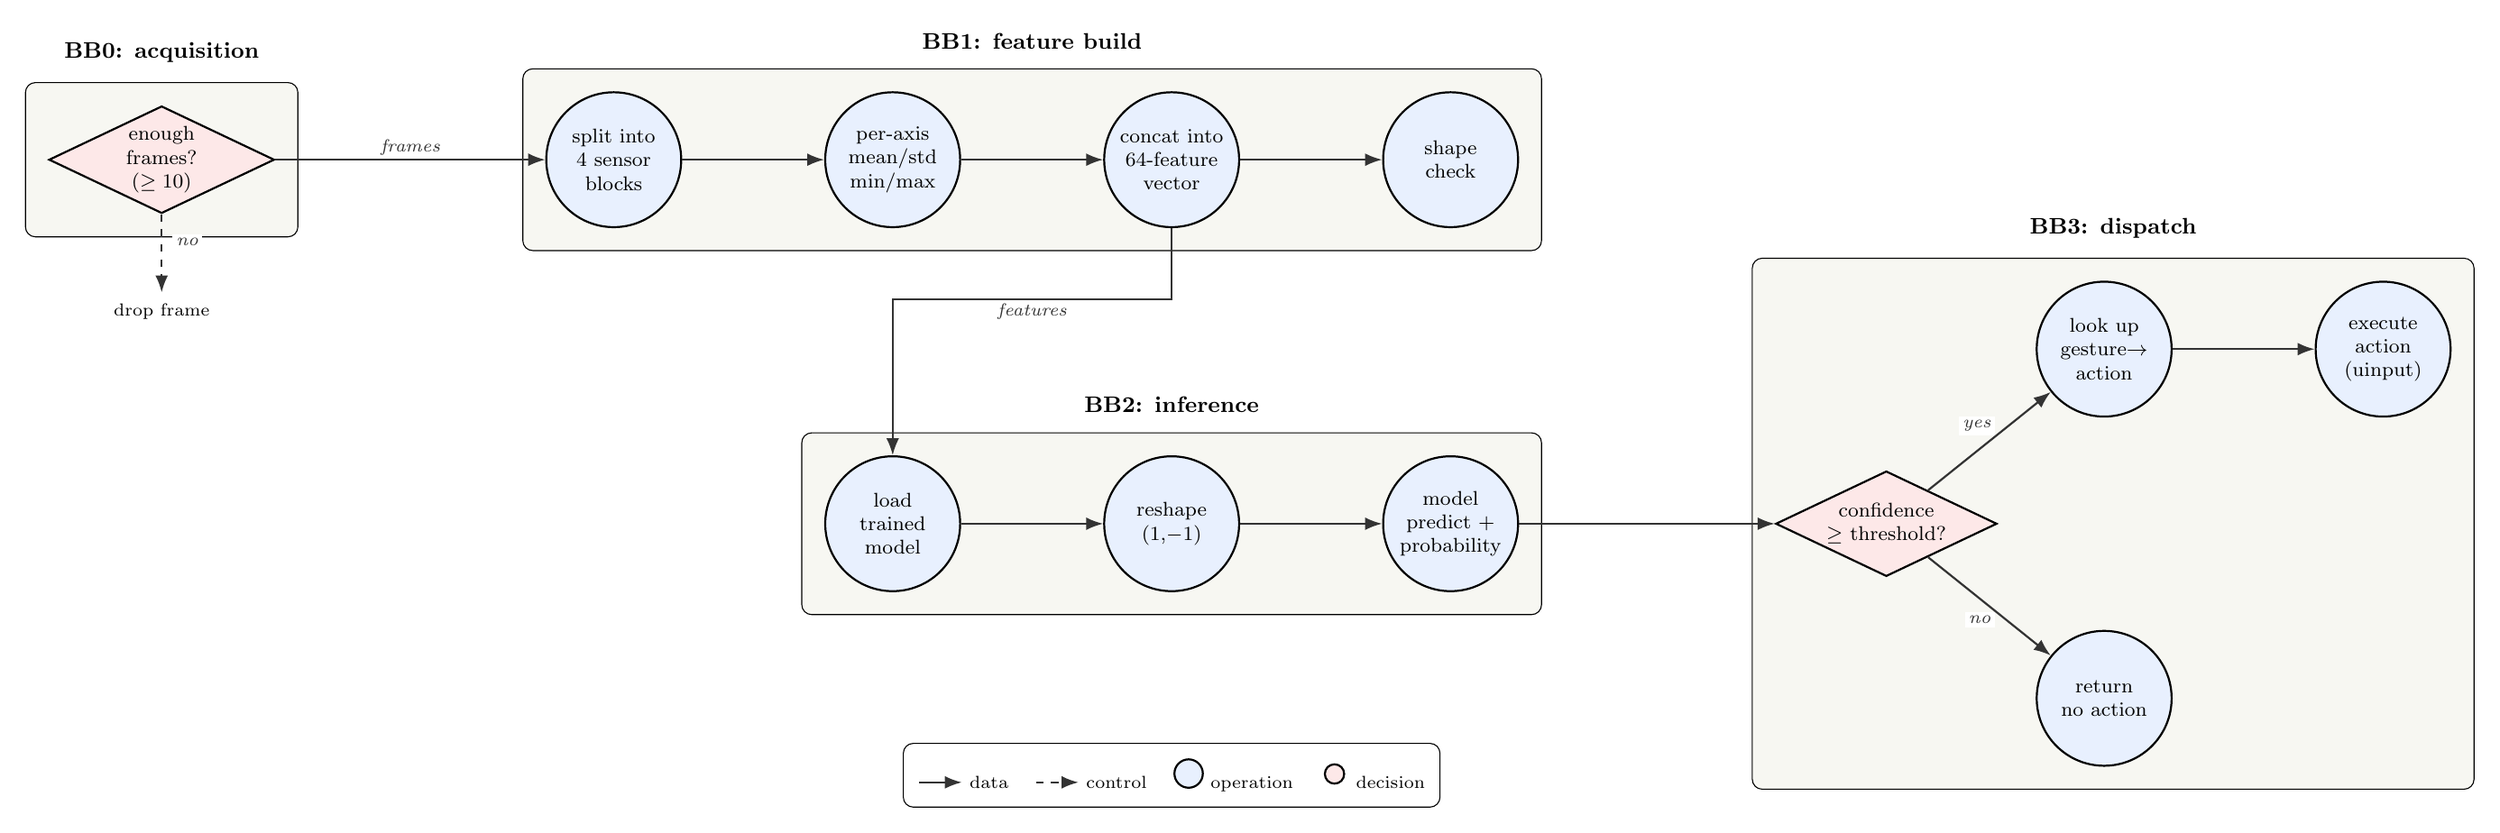
\begin{tikzpicture}[
  font=\footnotesize,
  node distance=18mm and 20mm,
  op/.style   ={circle, draw, thick, fill=opfill, minimum size=19mm, inner sep=1pt, align=center},
  dec/.style  ={diamond, draw, thick, fill=decfill, aspect=2.1, minimum width=24mm, inner sep=1pt, align=center},
  data/.style ={-{Latex[length=2.4mm]}, thick, draw=edge},
  ctrl/.style ={-{Latex[length=2.4mm]}, thick, dashed, draw=edge},
  elbl/.style ={font=\scriptsize\itshape, fill=white, inner sep=1.5pt, text=edge},
  bbstyle/.style={draw, rounded corners, fill=bb, inner sep=9pt}
]

% ================= BB0 : acquisition =================
\node[dec] (n1) {enough\\frames?\\$(\ge 10)$};

% ================= BB1 : feature build =================
\node[op, right=38mm of n1] (n4) {split into\\4 sensor\\blocks};
\node[op, right=of n4] (n5) {per-axis\\mean/std\\min/max};
\node[op, right=of n5] (n6) {concat into\\64-feature\\vector};
\node[op, right=of n6] (n7) {shape\\check};

% ================= BB2 : inference =================
\node[op, below=32mm of n5] (n8) {load\\trained\\model};
\node[op, right=of n8] (n9) {reshape\\(1,$-$1)};
\node[op, right=of n9] (n10) {model\\predict +\\probability};

% ================= BB3 : dispatch =================
\node[dec, right=36mm of n10] (n11) {confidence\\$\ge$ threshold?};
\node[op, above right=14mm and 16mm of n11] (n12) {look up\\gesture$\to$\\action};
\node[op, right=of n12] (n14) {execute\\action\\(uinput)};
\node[op, below right=14mm and 16mm of n11] (n13) {return\\no action};

% ================= data edges =================
\draw[data] (n1) -- node[elbl, above]{frames} (n4);
\draw[data] (n4) -- (n5);
\draw[data] (n5) -- (n6);
\draw[data] (n6) -- (n7);
\draw[data] (n6.south) -- ++(0,-10mm) -| node[elbl, pos=0.25, below]{features} (n8.north);
\draw[data] (n8) -- (n9);
\draw[data] (n9) -- (n10);
\draw[data] (n10) -- (n11);
\draw[data] (n11) -- node[elbl, pos=0.55, above left]{yes} (n12);
\draw[data] (n12) -- (n14);
\draw[data] (n11) -- node[elbl, pos=0.55, below left]{no} (n13);

% ================= control edge (drop) =================
\draw[ctrl] (n1.south) -- ++(0,-11mm) node[elbl, right=4pt, pos=0.35]{no} node[below=1pt, font=\scriptsize]{drop frame};

% ================= basic-block frames =================
\begin{scope}[on background layer]
  \node[bbstyle, fit=(n1)] (b0) {};
  \node[bbstyle, fit=(n4)(n5)(n6)(n7)] (b1) {};
  \node[bbstyle, fit=(n8)(n9)(n10)] (b2) {};
  \node[bbstyle, fit=(n11)(n12)(n14)(n13)] (b3) {};
\end{scope}
\node[above=1.5mm of b0.north, font=\small\bfseries] {BB0: acquisition};
\node[above=1.5mm of b1.north, font=\small\bfseries] {BB1: feature build};
\node[above=1.5mm of b2.north, font=\small\bfseries] {BB2: inference};
\node[above=1.5mm of b3.north, font=\small\bfseries] {BB3: dispatch};

% ================= legend =================
\node[draw, rounded corners, fill=white, below=18mm of b2.south, anchor=north, inner sep=6pt, font=\scriptsize] (leg) {
  \tikz\draw[data] (0,0)--(6mm,0); data \quad
  \tikz\draw[ctrl] (0,0)--(6mm,0); control \quad
  \tikz\node[op,minimum size=4mm,inner sep=0]{};
  operation \quad
  \tikz\node[dec,minimum size=4mm,aspect=2,inner sep=0]{};
  decision};

\end{tikzpicture}
\end{document}
